\documentclass[12pt]{article}
\usepackage{amsmath}
\usepackage[top=0.9in, bottom=0.9in, left=0.8in, right=0.5in]{geometry}

\usepackage{caption}
\usepackage{float}
\usepackage{graphicx}
\usepackage{subfig}
\usepackage{wrapfig,lipsum}
\usepackage{amssymb}
\usepackage{nath}
\usepackage{amsfonts}
\usepackage{float}
\usepackage{hhline}
\begin{document}

\title{MAT160 - Final Project}
\author{Ahmed H. Mahmoud}
\date{June, 11th 2017} 

\maketitle

\newcommand{\cn}{Crank-Nicolson}


%============Table========
%\begin{figure}[tbh]
% \centering    
%\begin{tabular}{ |p{4cm}|| p{2cm}|p{2cm}|p{2cm}|p{2cm}|}
% \hline
% & Processor 1 &  Processor 2  & Processor 3 & Processor 4\\ \hhline{|=|=|=|=|=|}
% \hline
% Performance          &$1.08$        &$1.425$       &\textbf{1.52}  &   \\
% \hline
%\end{tabular} 
%\caption{Metric table for the four processors}
%   \label{tab:metric}
%\end{figure} 
%============Figure========
%\begin{figure}[!tbh]
%\centering        
%   \subfloat {\includegraphics[width=0.65\textwidth]{fig2_4.png}}
%   \caption{ }
%   \label{fig:fig}
%\end{figure}


\section*{Problem No.1} \label{sec:prob1}
\paragraph{Part A:}
Our code consists of first computing the left $K$ singular vectors or rank $K$ approximation $U_{k}^{(j)}$ ($j$ represents the class) using the MATLAB function $\mathtt{svds}$ for each class $X^{(j)}$ using the training data set. For each test data point $y_{i}$, we compare the data point with all computed singular vectors (10 classes) and the inference value of the data point is the class of minimal error. The error of data point $y_{i}$ w.r.t class $j$ is computed as $E_{j}y_{i}=||y_{i}-U_{k}^{(j)}(U_{k}^{(j)T}y_{i}) ||_{2}$. Figure \ref{fig:svd} shows the first five left singular vectors plotted as images for the first three classes (digits 0, 1 and 2). We notice that the first left singular vector (associated with largest singular value) closely resemble the corresponding digit followed by the second singular vector. 


\begin{figure}[!tbh]
\centering        
   \subfloat {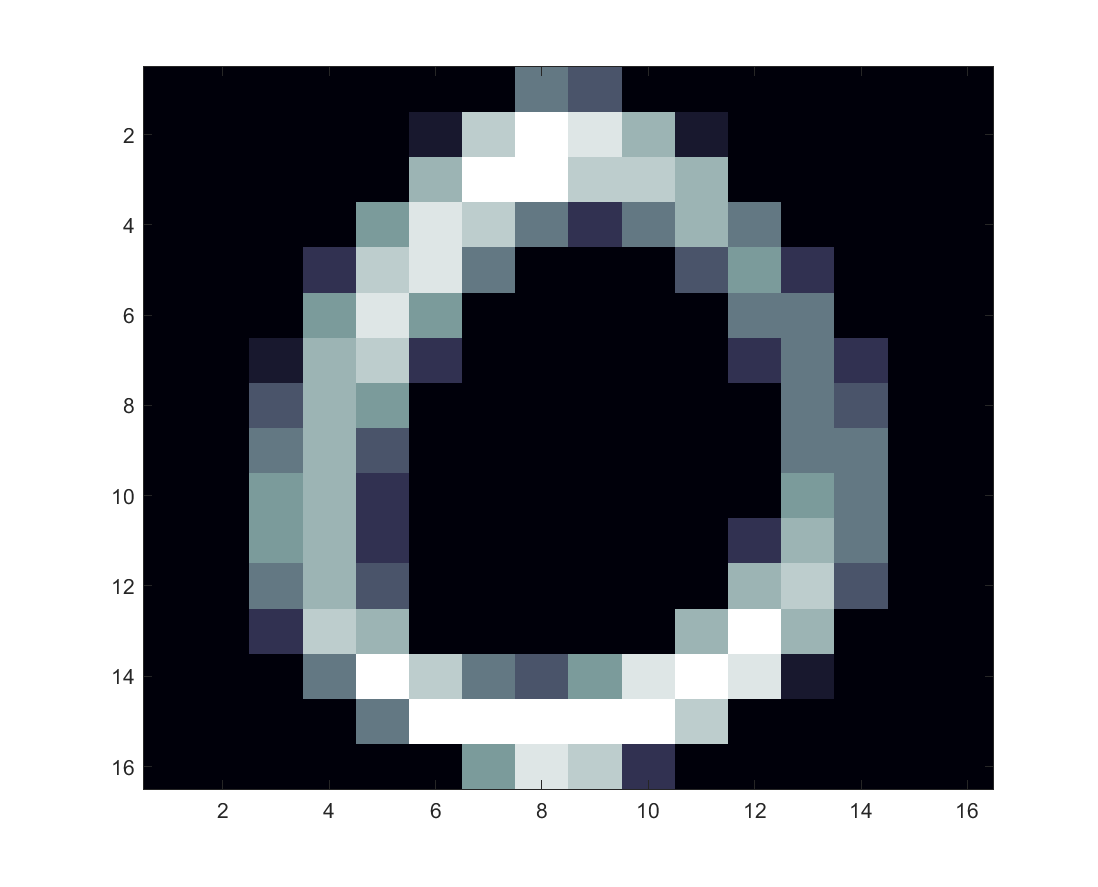
\includegraphics[width=0.2\textwidth]{fig/class_1_K1.png}}
   \subfloat {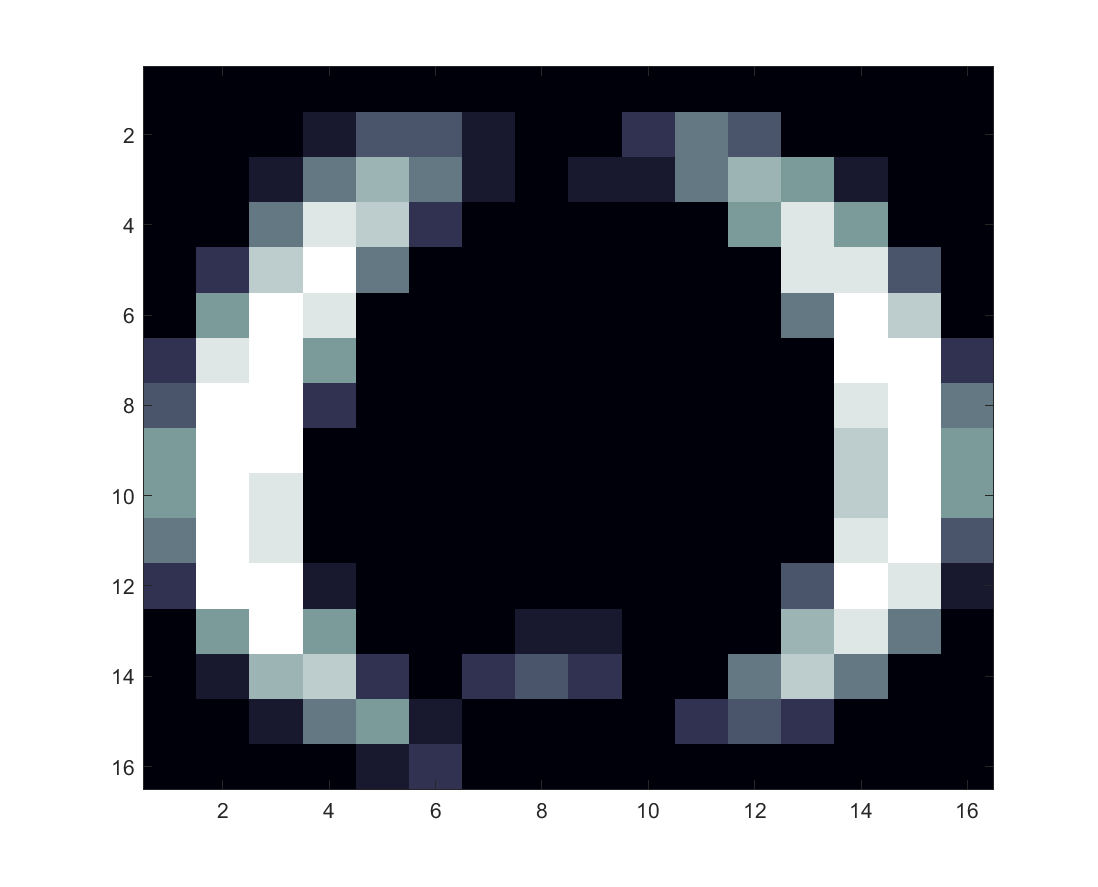
\includegraphics[width=0.2\textwidth]{fig/class_1_K2.png}}
   \subfloat {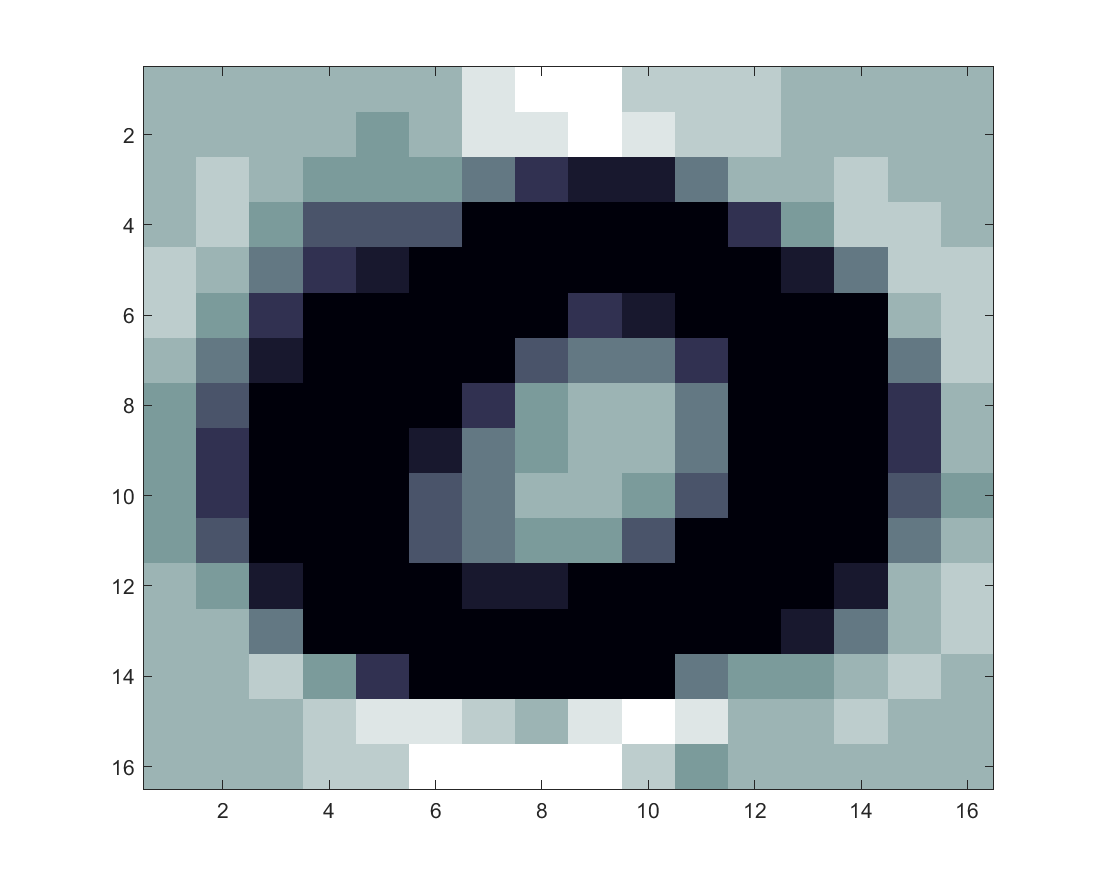
\includegraphics[width=0.2\textwidth]{fig/class_1_K3.png}}
   \subfloat {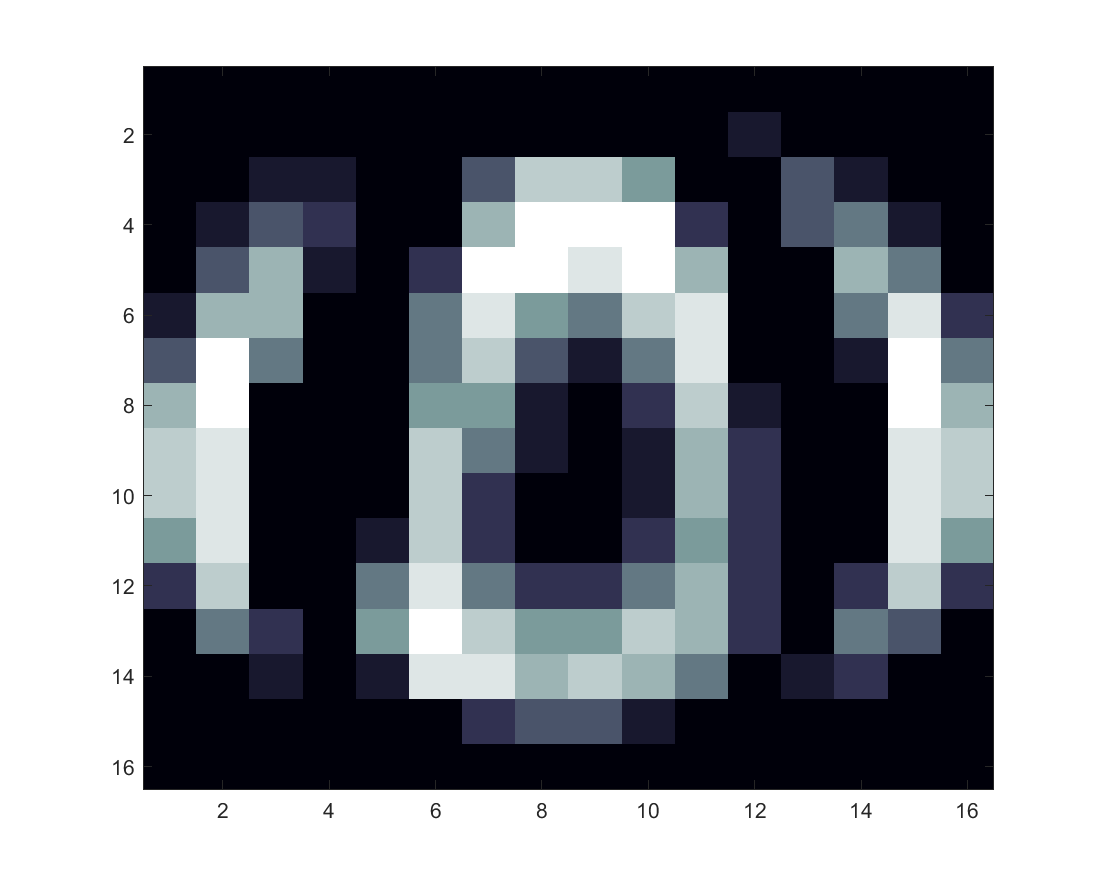
\includegraphics[width=0.2\textwidth]{fig/class_1_K4.png}}
   \subfloat {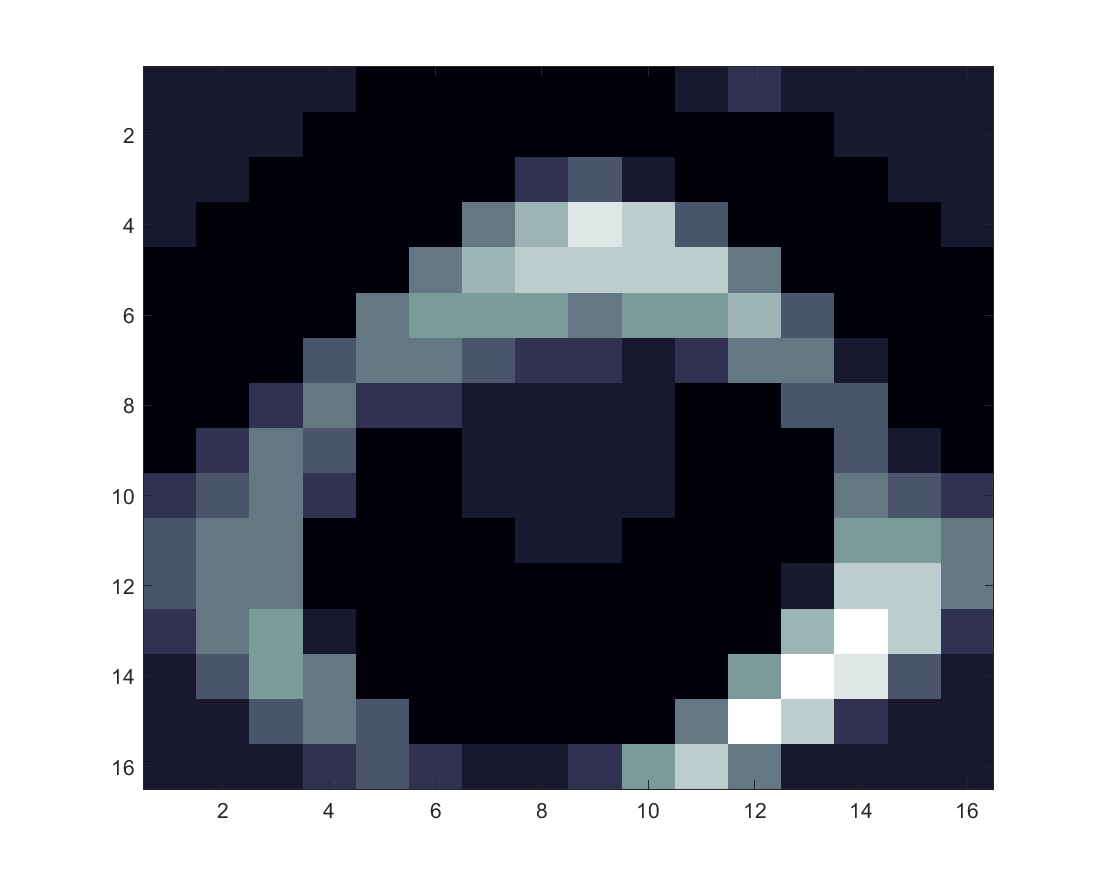
\includegraphics[width=0.2\textwidth]{fig/class_1_K5.png}}
   
   \subfloat {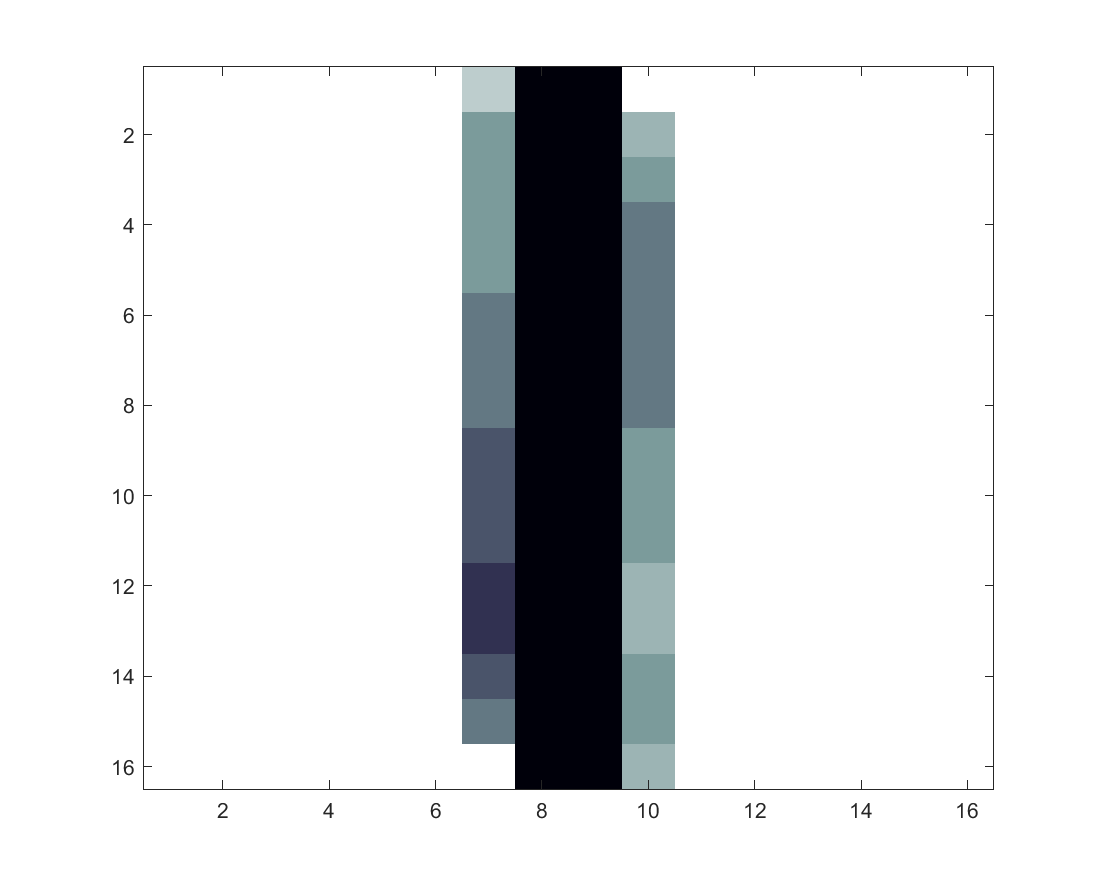
\includegraphics[width=0.2\textwidth]{fig/class_2_K1.png}}
   \subfloat {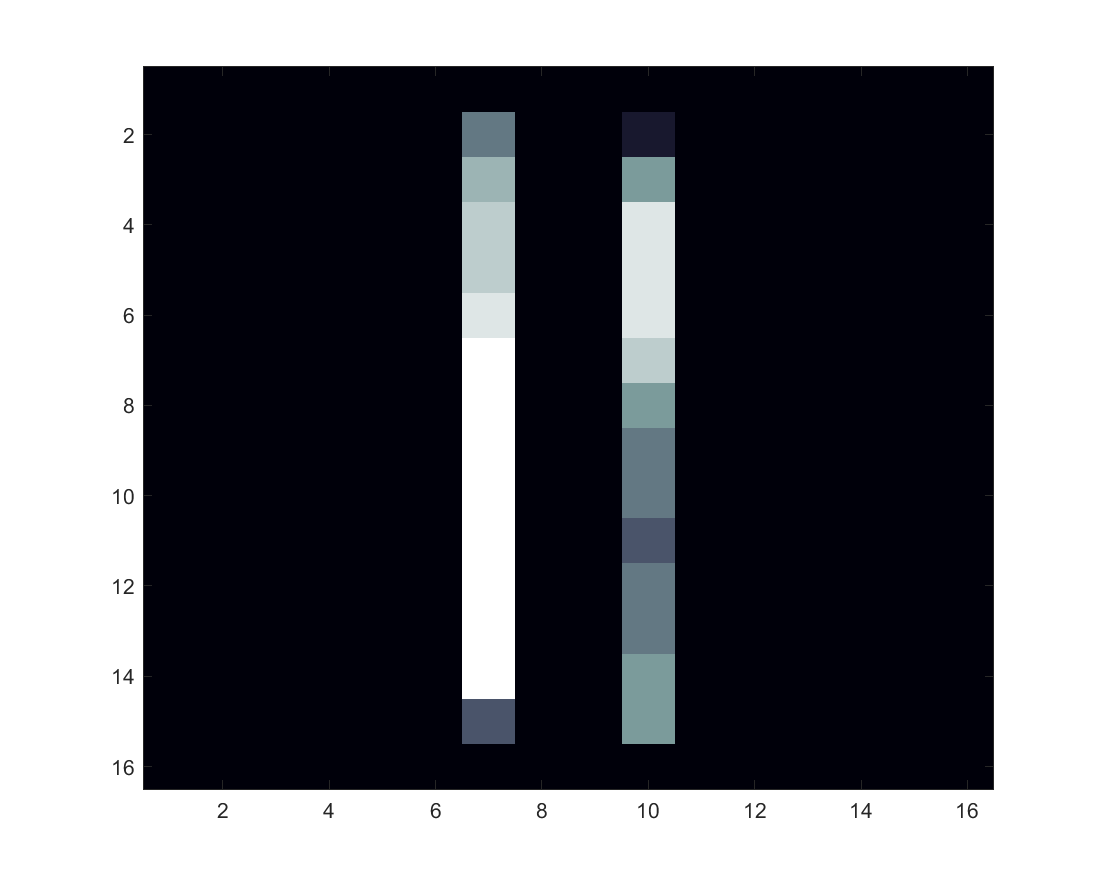
\includegraphics[width=0.2\textwidth]{fig/class_2_K2.png}}
   \subfloat {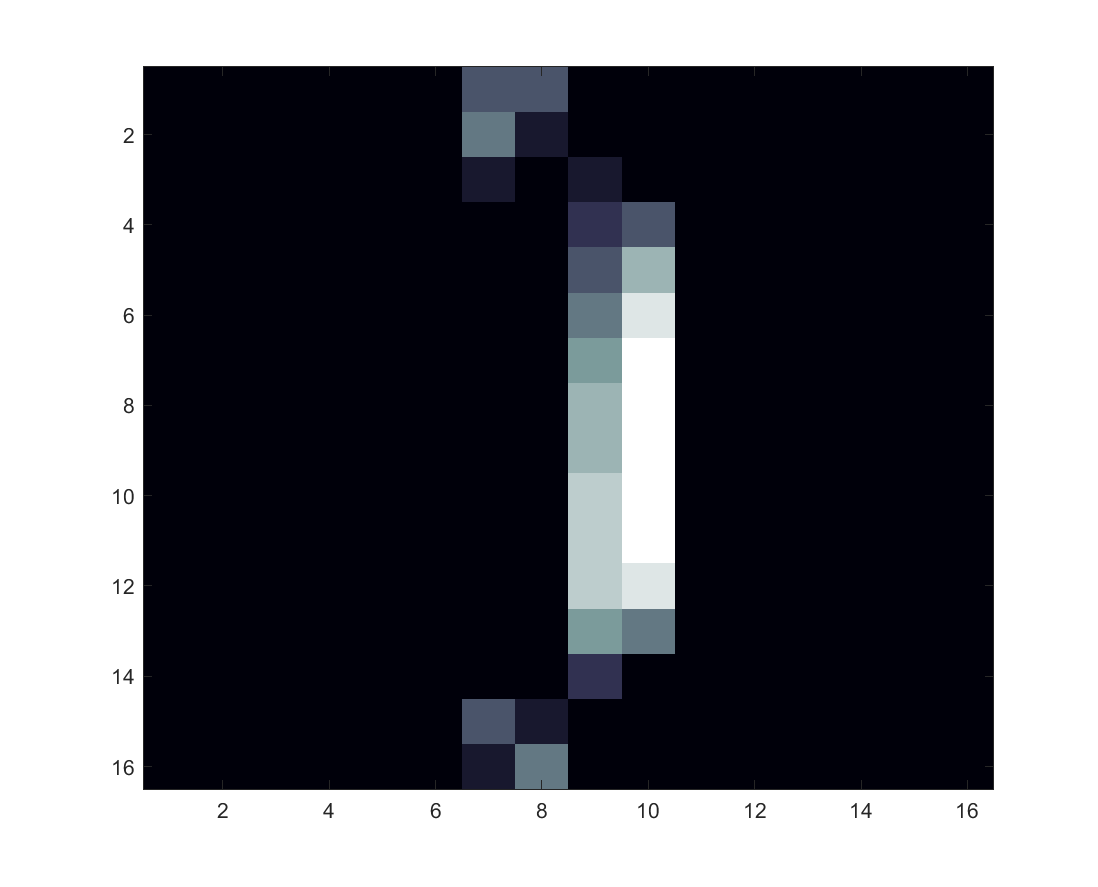
\includegraphics[width=0.2\textwidth]{fig/class_2_K3.png}}
   \subfloat {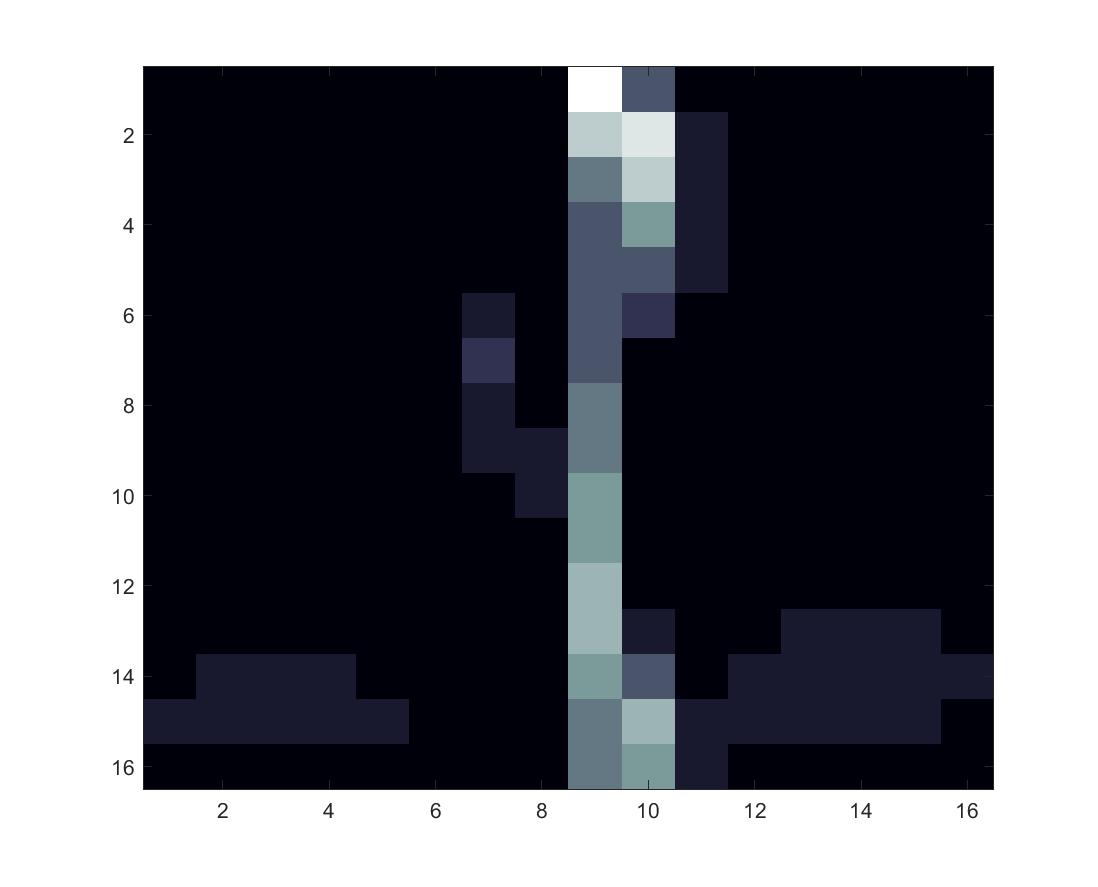
\includegraphics[width=0.2\textwidth]{fig/class_2_K4.png}}
   \subfloat {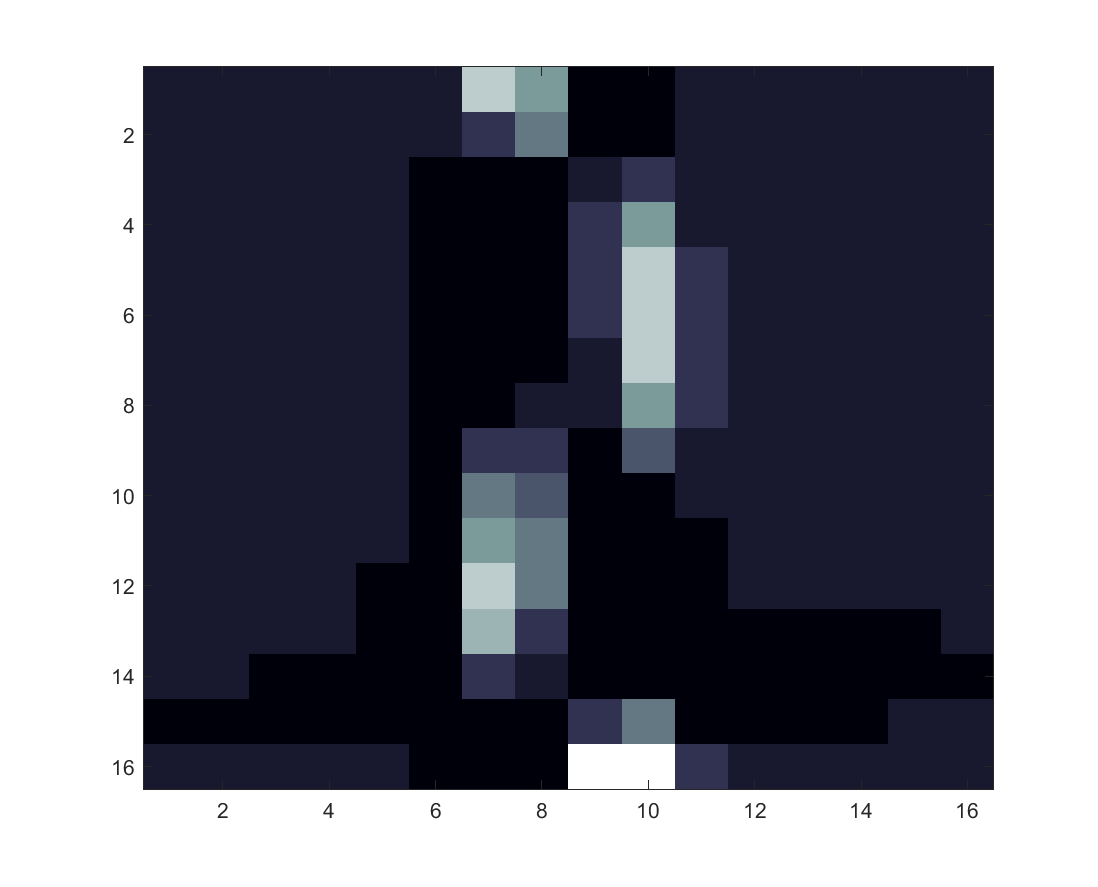
\includegraphics[width=0.2\textwidth]{fig/class_2_K5.png}}
   
   \subfloat {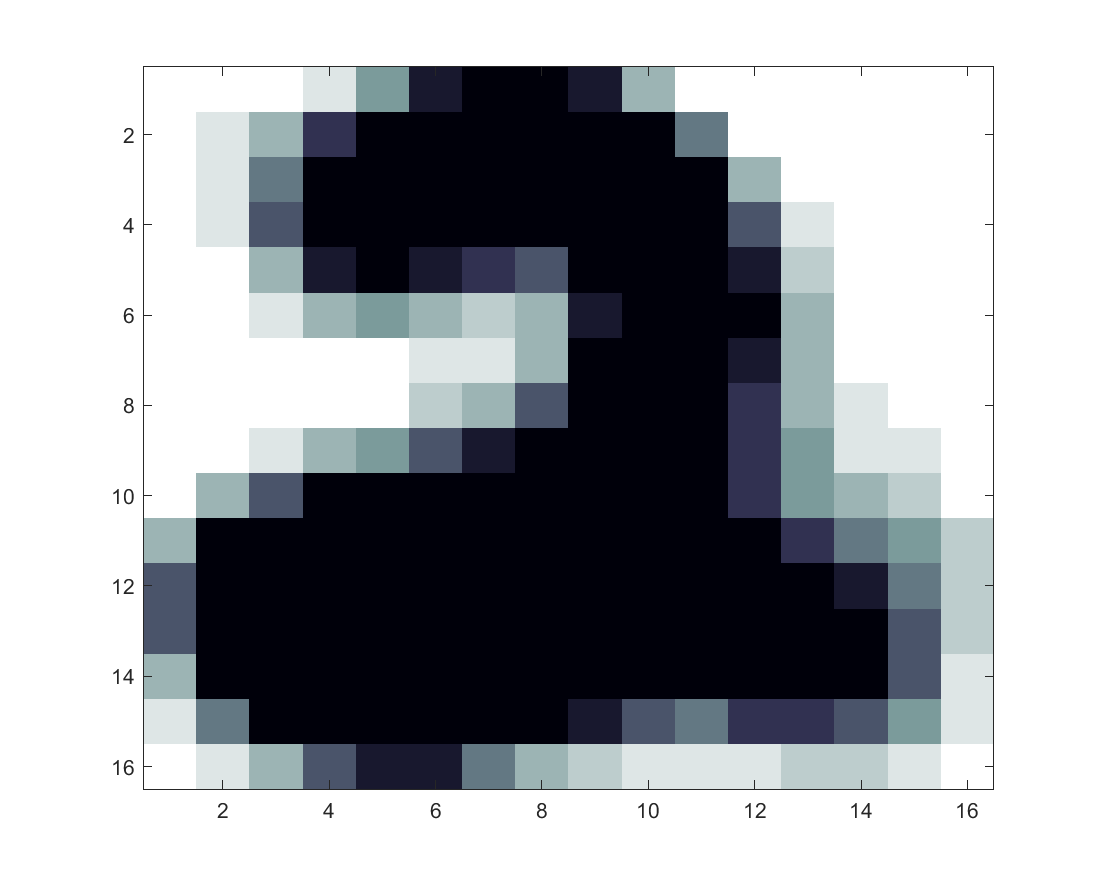
\includegraphics[width=0.2\textwidth]{fig/class_3_K1.png}}
   \subfloat {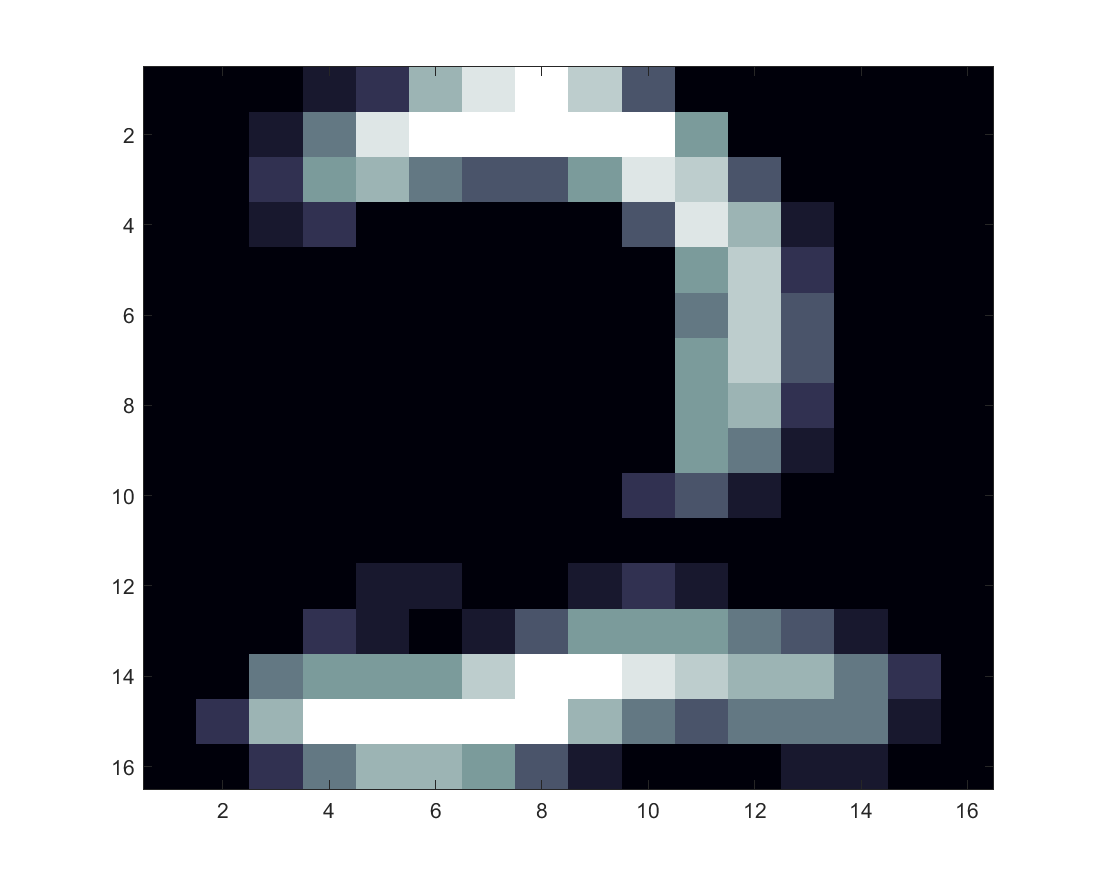
\includegraphics[width=0.2\textwidth]{fig/class_3_K2.png}}
   \subfloat {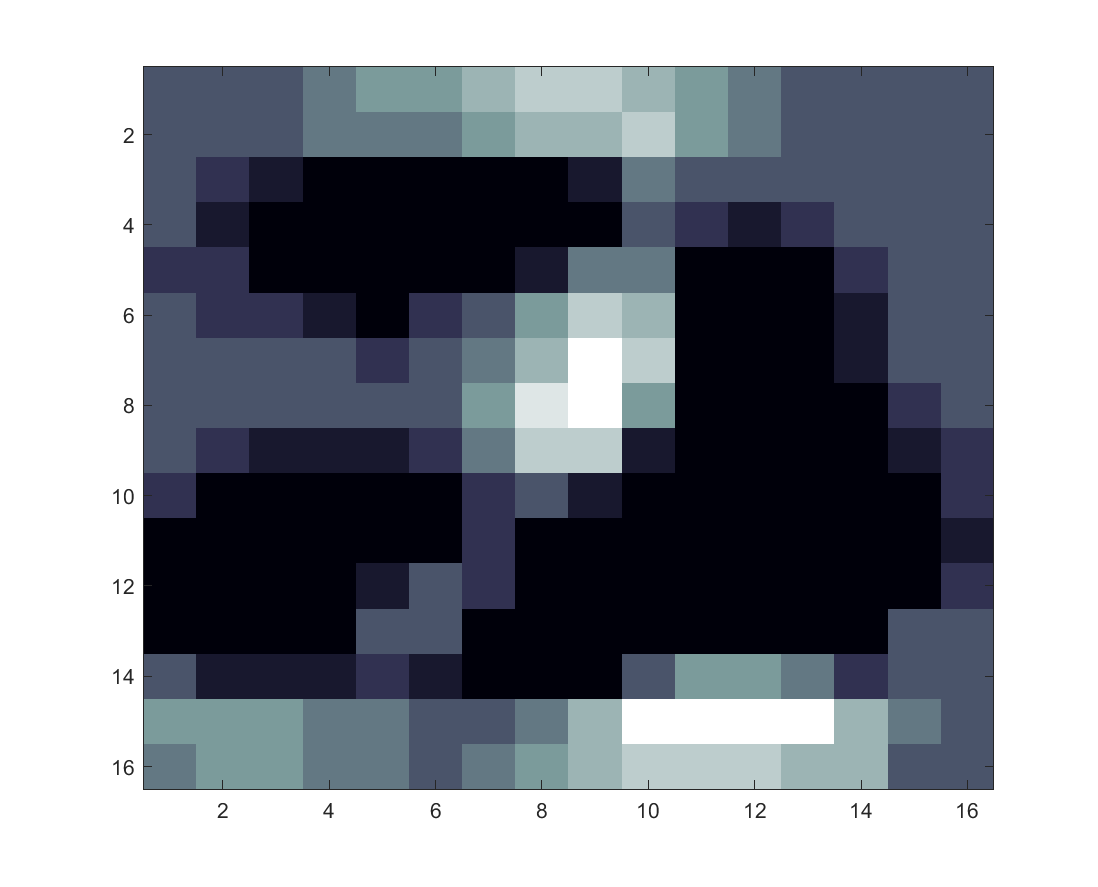
\includegraphics[width=0.2\textwidth]{fig/class_3_K3.png}}
   \subfloat {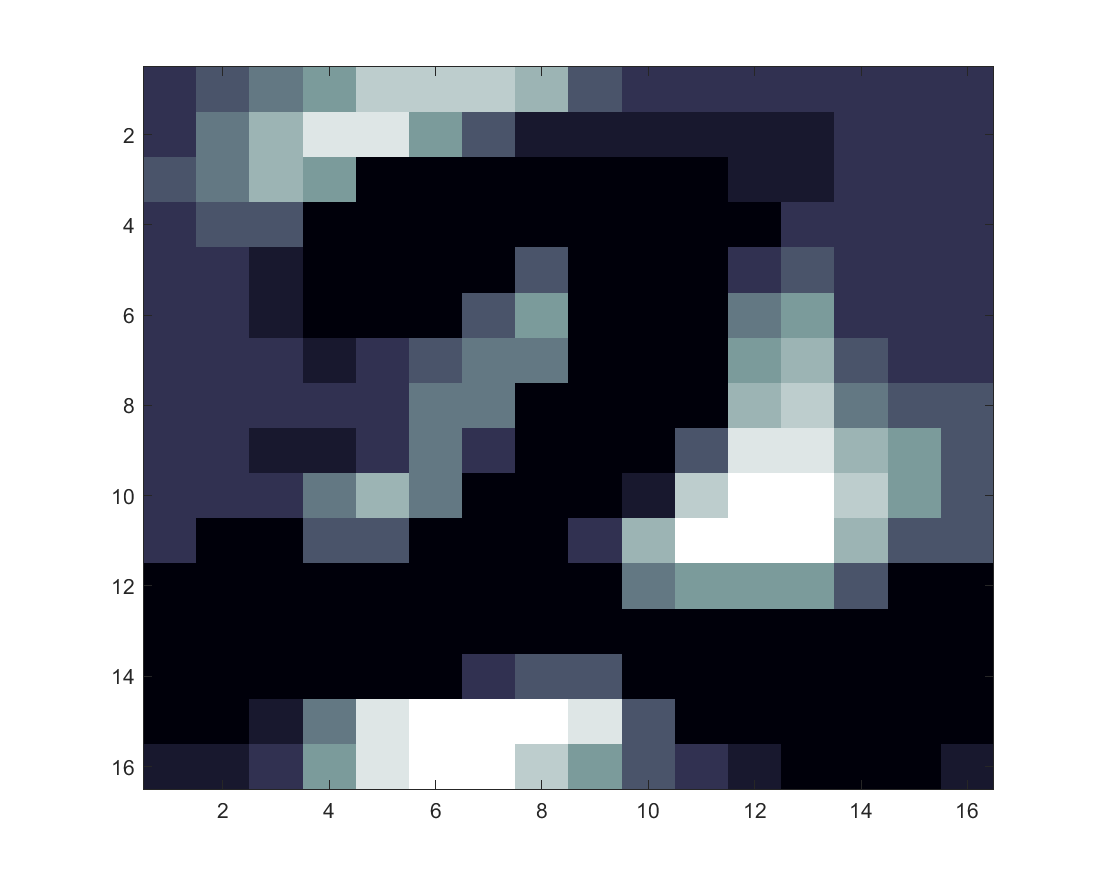
\includegraphics[width=0.2\textwidth]{fig/class_3_K4.png}}
   \subfloat {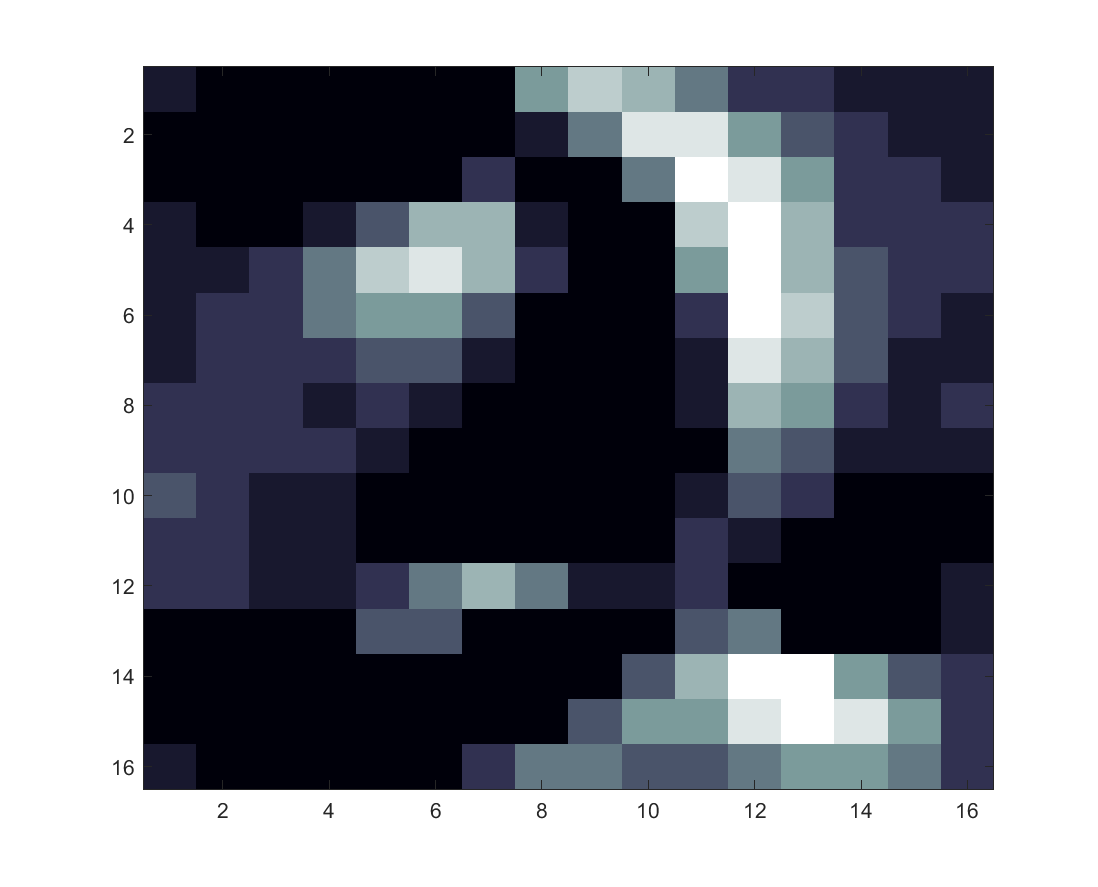
\includegraphics[width=0.2\textwidth]{fig/class_3_K5.png}}
   
   %\subfloat {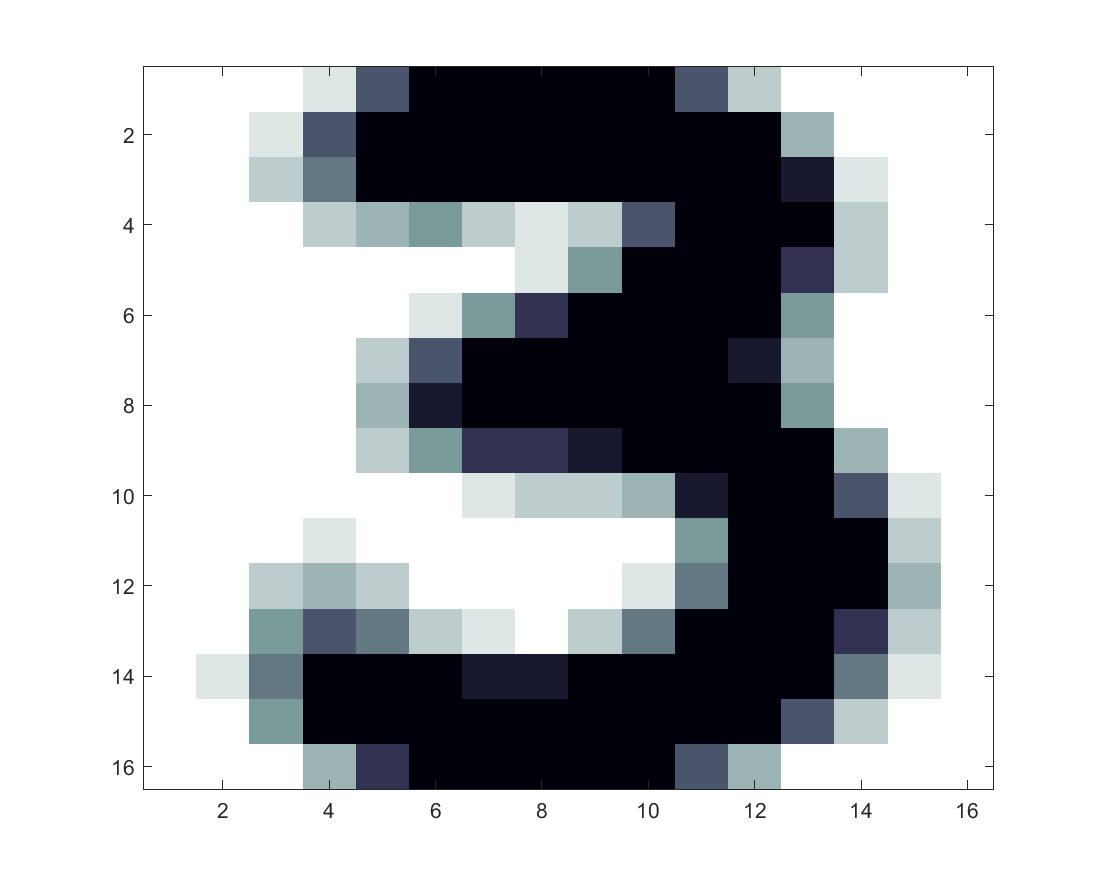
\includegraphics[width=0.2\textwidth]{fig/class_4_K1.png}}
   %\subfloat {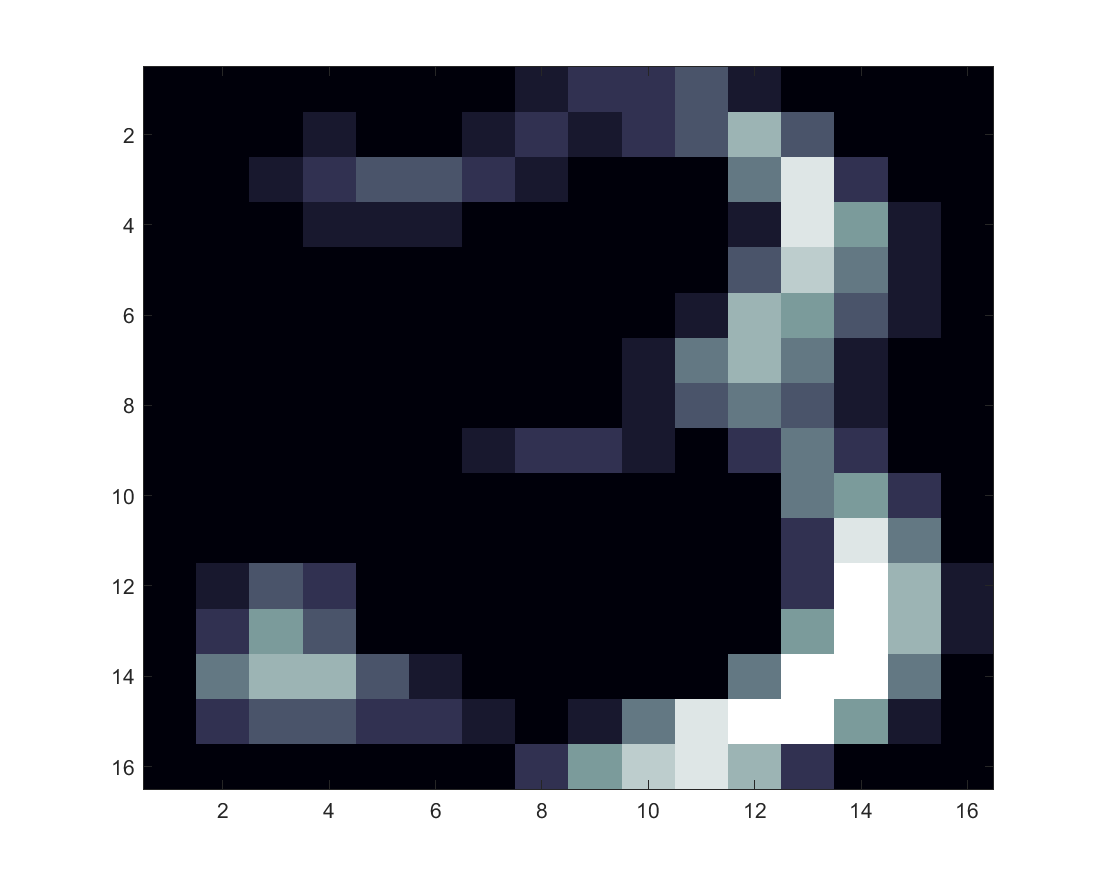
\includegraphics[width=0.2\textwidth]{fig/class_4_K2.png}}
   %\subfloat {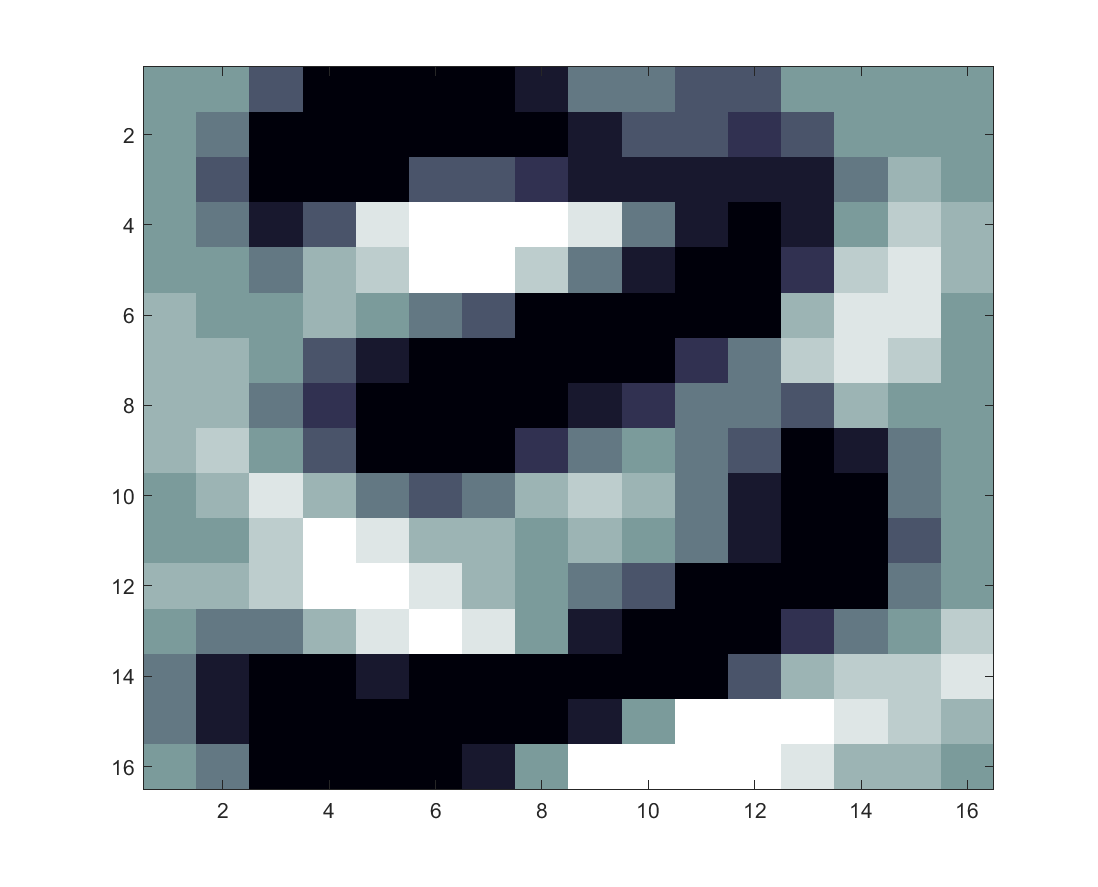
\includegraphics[width=0.2\textwidth]{fig/class_4_K3.png}}
   %\subfloat {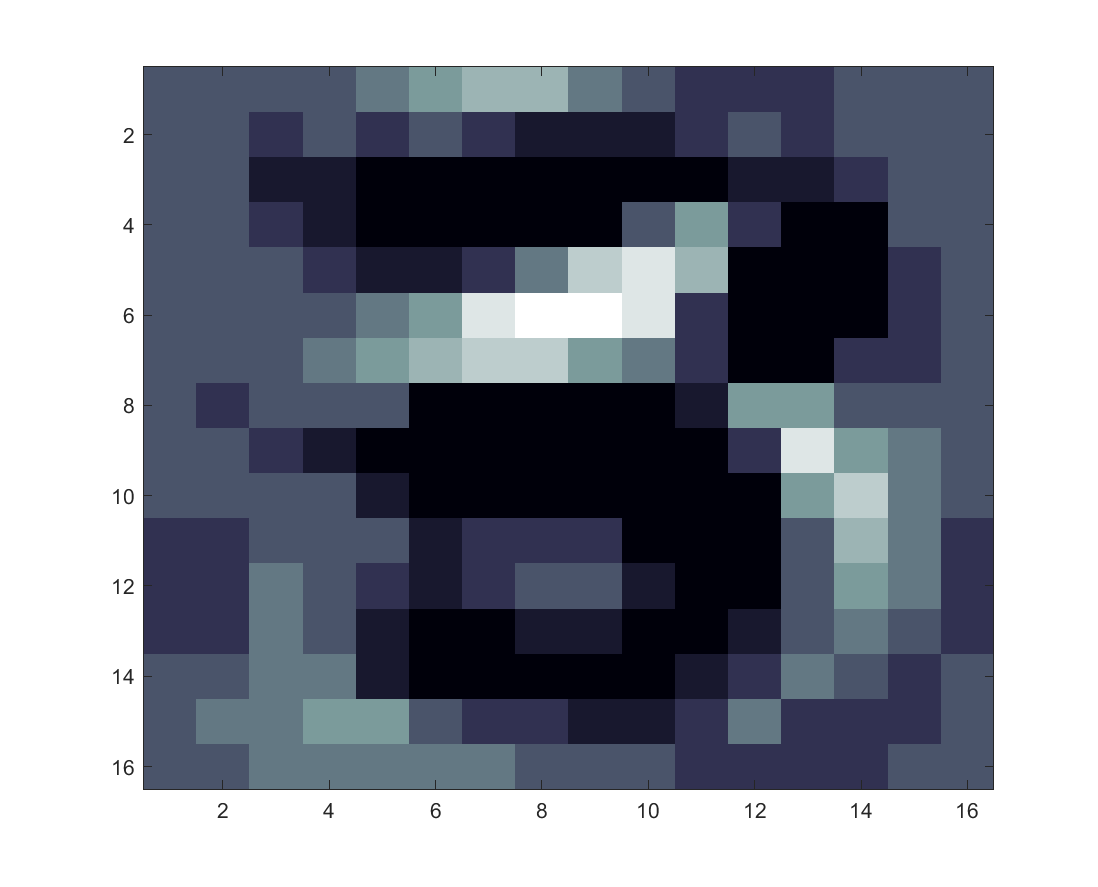
\includegraphics[width=0.2\textwidth]{fig/class_4_K4.png}}
   %\subfloat {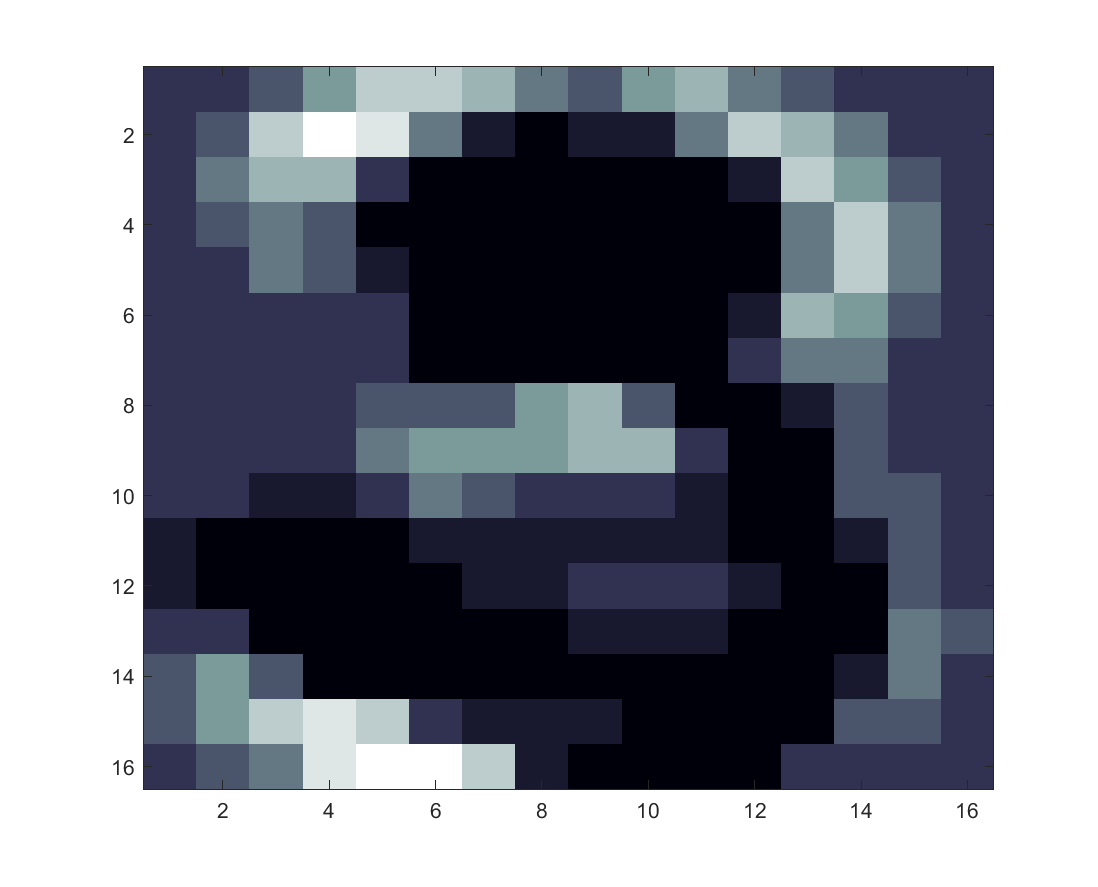
\includegraphics[width=0.2\textwidth]{fig/class_4_K5.png}}
   
   %\subfloat {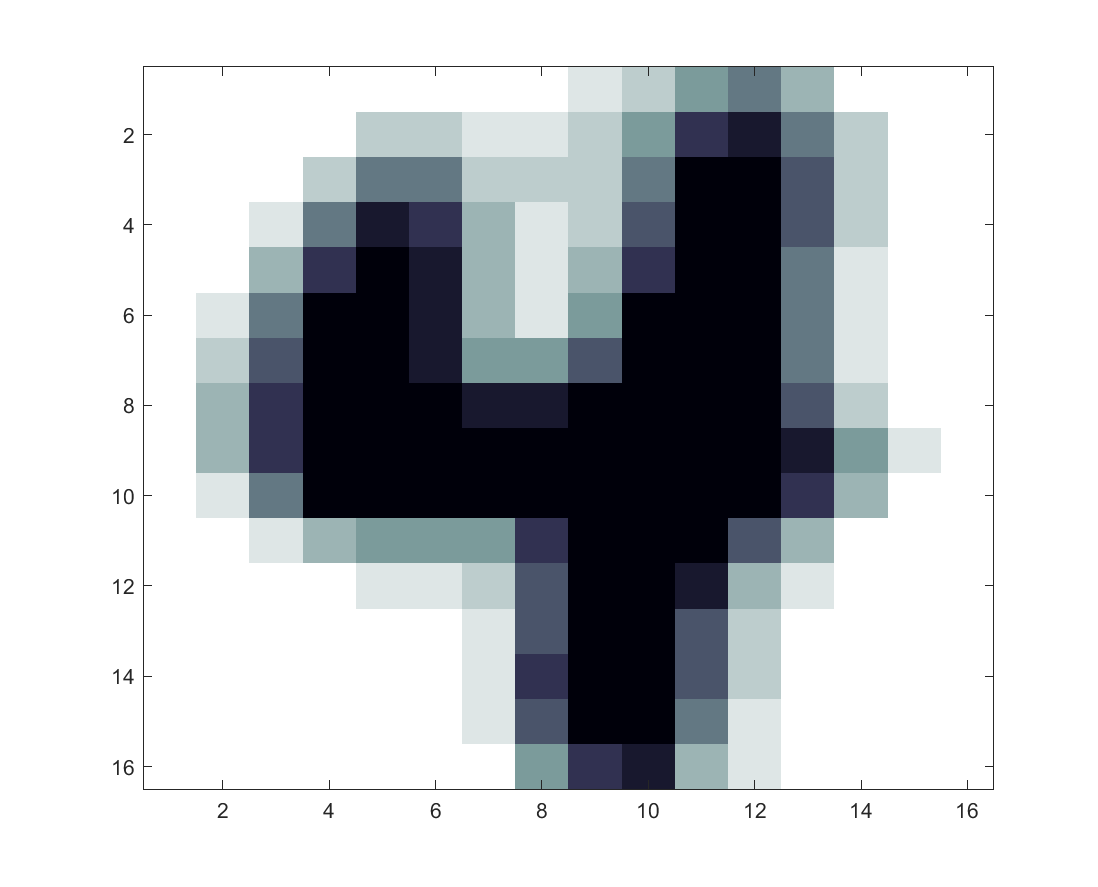
\includegraphics[width=0.2\textwidth]{fig/class_5_K1.png}}
   %\subfloat {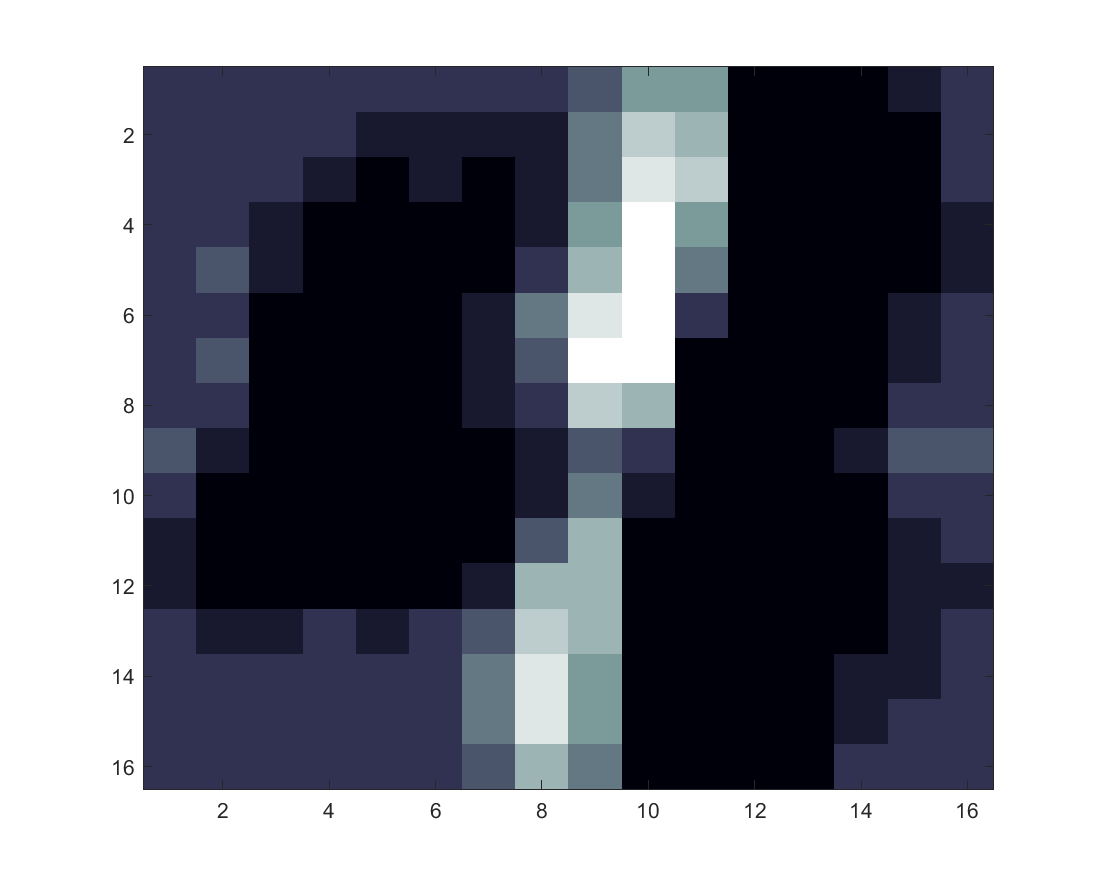
\includegraphics[width=0.2\textwidth]{fig/class_5_K2.png}}
   %\subfloat {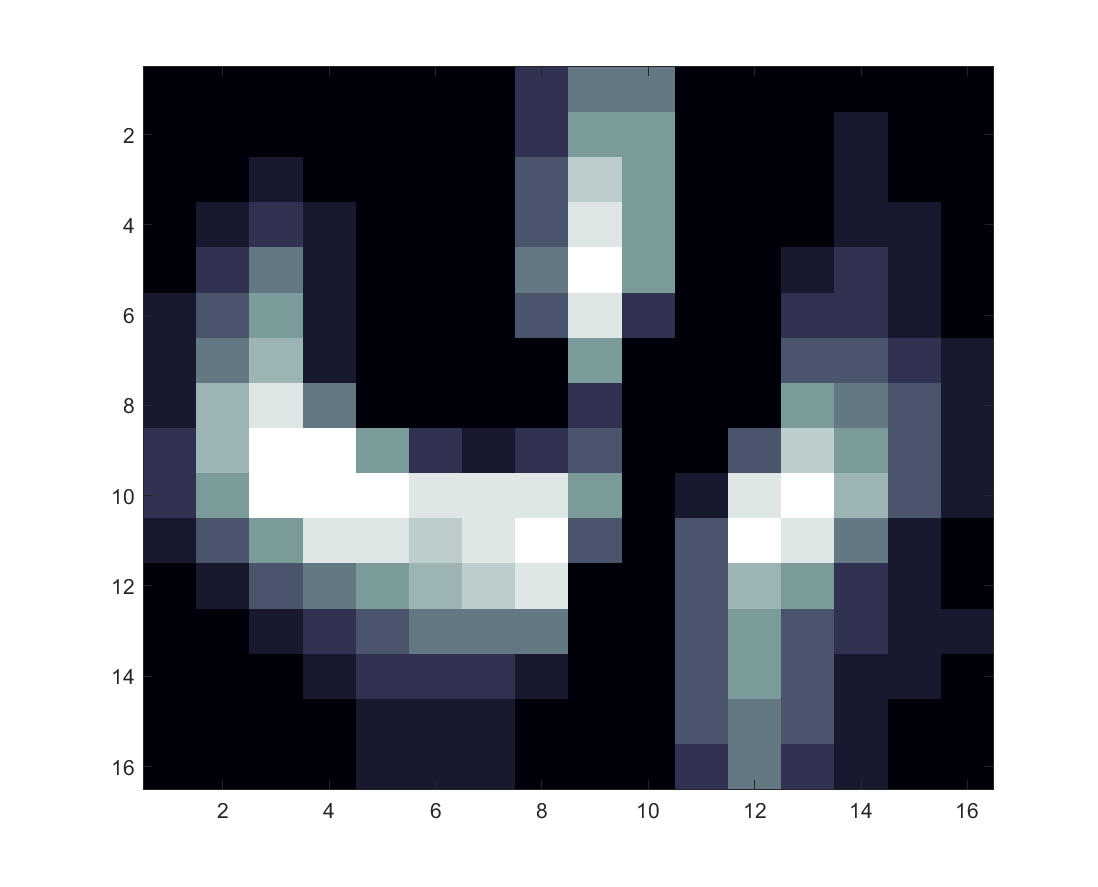
\includegraphics[width=0.2\textwidth]{fig/class_5_K3.png}}
   %\subfloat {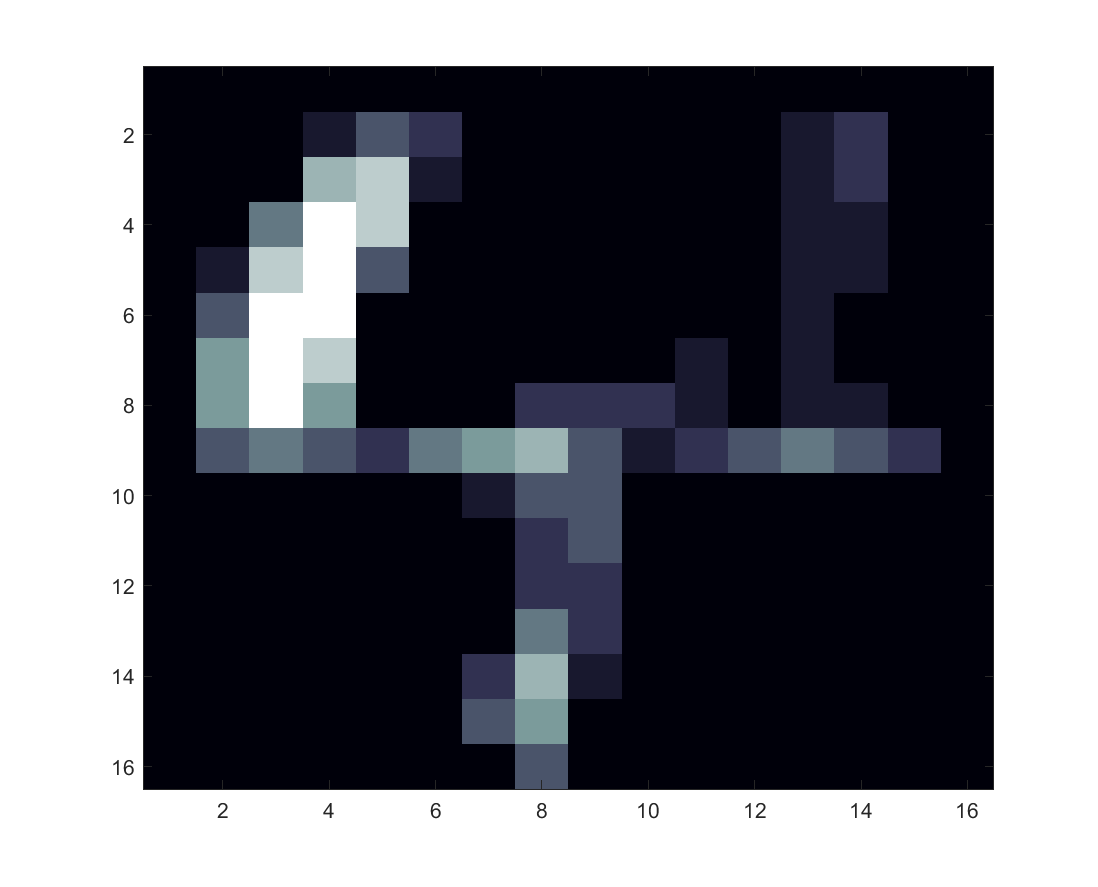
\includegraphics[width=0.2\textwidth]{fig/class_5_K4.png}}
   %\subfloat {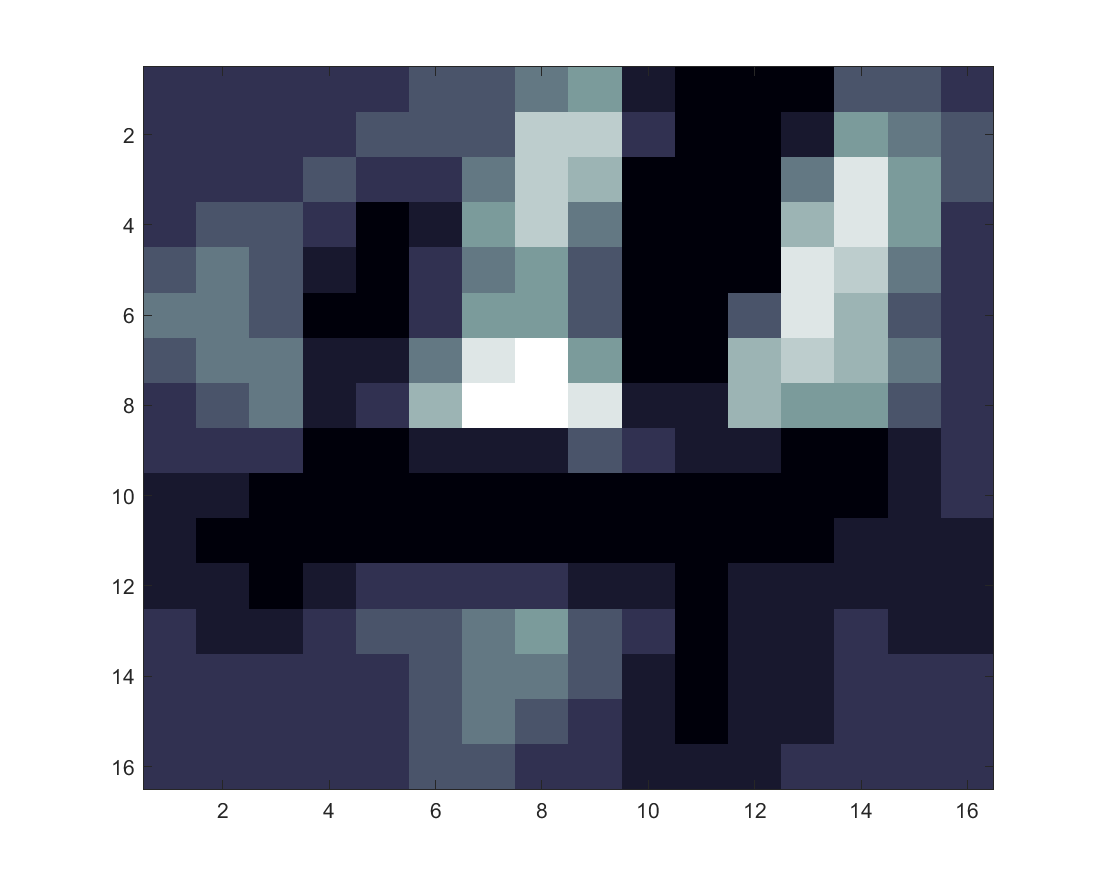
\includegraphics[width=0.2\textwidth]{fig/class_5_K5.png}}
   
   \caption{ First left (associated with largest singular values) singular vectors for the first three classes.}
   \label{fig:svd}
\end{figure}




\vspace{-6.5mm}
\begin{wrapfigure}[6]{r}{65mm}
  \begin{center}
	\begin{tabular}{|c||p{1.6cm}|}
	 \hline
  \# Basis Vector & Accuracy   \\ \hhline{|=|=|}\hline
   5 &90.3\% \\
   \hline
   10 &93.2\% \\
  \hline
   20 & 93.9 \%\\
	\hline
	\end{tabular} 
 	%\caption*{Incidence/Adjacent Table}
  \end{center} 
\end{wrapfigure}


\paragraph{Part B:}
We computed the accuracy as a function of the number of basis vector $K$. The accuracy is computed as the percentage of the number of images that has been classified correctly to all images that has been tested. Figure~\ref{fig:acc}(a) shows the relation between accuracy and the number of basis vector. The maximum accuracy \textbf{94.32\%} with \textbf{22} basis vector.  The table to the right show the accuracy values for 5, 10, and 20 basis vector. 

\begin{figure}[!tbh]
\centering        
   \subfloat []{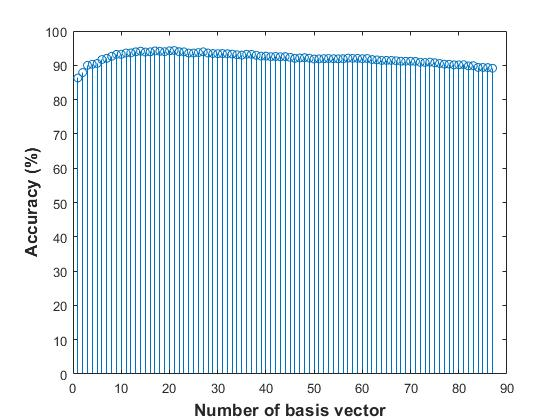
\includegraphics[width=0.5\textwidth]{fig/acc.jpg}}
   \subfloat []{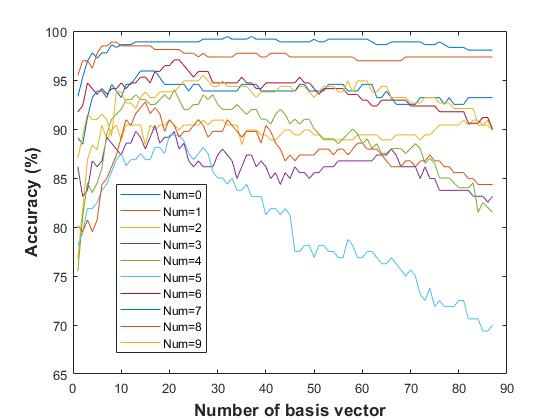
\includegraphics[width=0.5\textwidth]{fig/acc_class.jpg}}
   \caption{The accuracy of classified images as a function of the number of basis vectors $K$ (a) for all images (b) per class/number.}
   \label{fig:acc}
\end{figure}

\paragraph{Part C \& D:}
In order to realize if it is beneficial to use different number of basis vector for different classes, we compute per-class accuracy for number of basis vector (from 2 up to 88). Figure~\ref{fig:acc}(b) shows the per-class accuracy for different basis vector. We can see for class of \textit{Number 5}, the accuracy decreases with increasing the number of basis vectors. For other classes like \textit{Number 0} and \textit{Number 1} the accuracy stays same (or marginally decreases) as the number of basis increases. For class of \textit{Number 5}, it is better to use 21 vector basis for which the accuracy is  89.3\%. Table~\ref{tab:acc} shows the maximum accuracy obtained for all class along with the number of basis vector associated with the maximum accuracy. We notice that class of \textit{Number 1} only need 9 basis vector due to symmetry and simplicity of the shape of number one, while \textit{Number 9} need up to 28 basis vector as it is not symmetric and the most complex. 

In order to investigate the class of \textit{Number 9} more thoroughly, we draw the few instances for which the number got mis-predicated using 28 basis vector as shown in Figure~\ref{fig:nine}. Most of the mis-predicated images are indeed badly written and looks likes other number like the first row in Figure~\ref{fig:nine} where the number looks more like \textit{Number 4} more than \textit{Number 9}.


\begin{figure}[tbh]
 \centering    
\begin{tabular}{ |c||c|c|}
 \hline
Class &  Max Accuracy (\%) &  \# Basis Vector   \\ \hhline{|=|=|=|}
 \hline
 \textit{Number 0}   & 99.4429 & 33\\
 \textit{Number 1}   & 98.8636 & 9 \\
 \textit{Number 2}   & 90.9091 & 21\\
 \textit{Number 3}   & 90.3614 & 18\\
 \textit{Number 4}   & 94.0000 & 22\\
 \textit{Number 5}   & 89.3750 & 21\\
 \textit{Number 6}   & 97.0588 & 22\\     
 \textit{Number 7}   & 95.9184 & 15\\
 \textit{Number 8}   & 92.7711 & 16\\
 \textit{Number 9}   & 95.4802 & 28\\      
 \hline
\end{tabular} 
\caption{The maximum accuracy obtained per class by varying the number of basis vectors. For each class, we report here the maximum accuracy along with the number of basis vector associated with it.}
   \label{tab:acc}
\end{figure} 



\begin{figure}[!tbh]
\centering        
   \subfloat [pred=4]{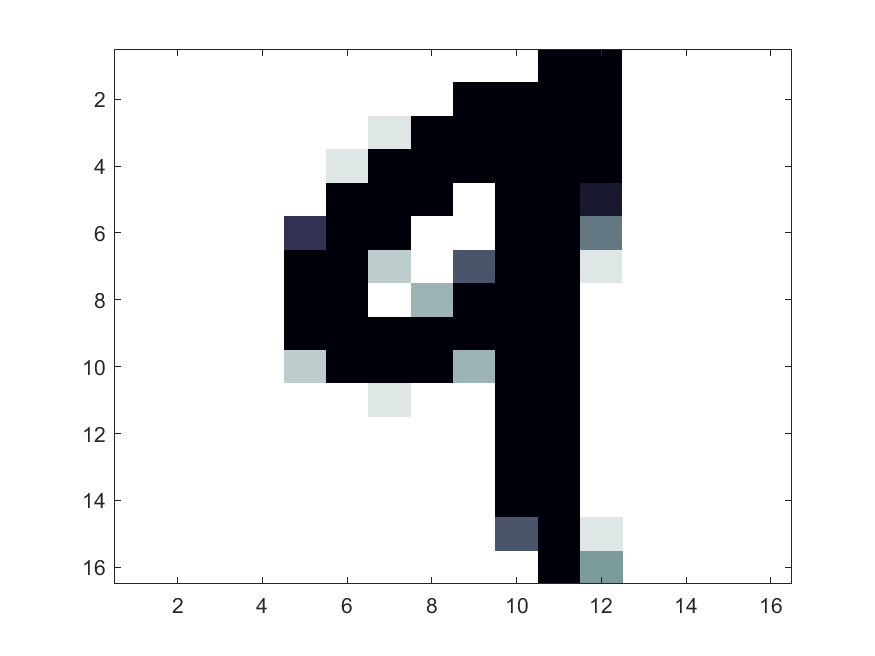
\includegraphics[width=0.25\textwidth]{fig/nine4_4.png}}
   \subfloat [pred=4]{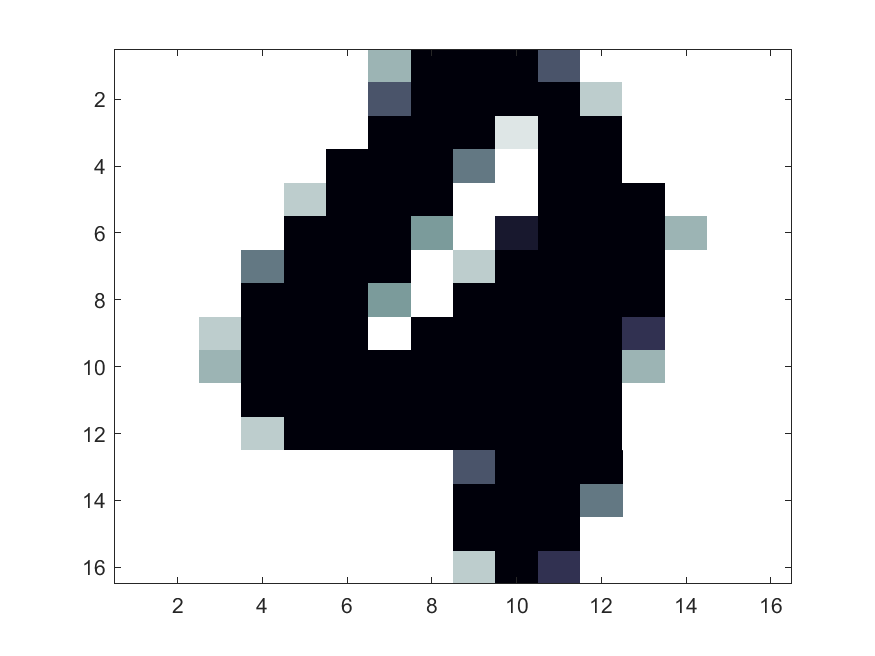
\includegraphics[width=0.25\textwidth]{fig/nine6_4.png}}
   \subfloat [pred=4]{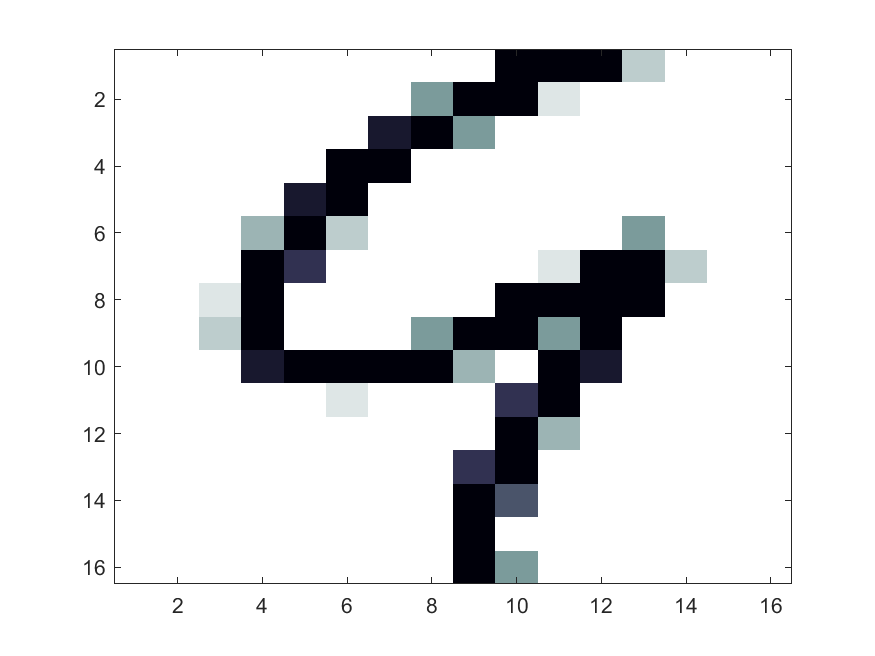
\includegraphics[width=0.25\textwidth]{fig/nine7_4.png}}
   \subfloat [pred=4]{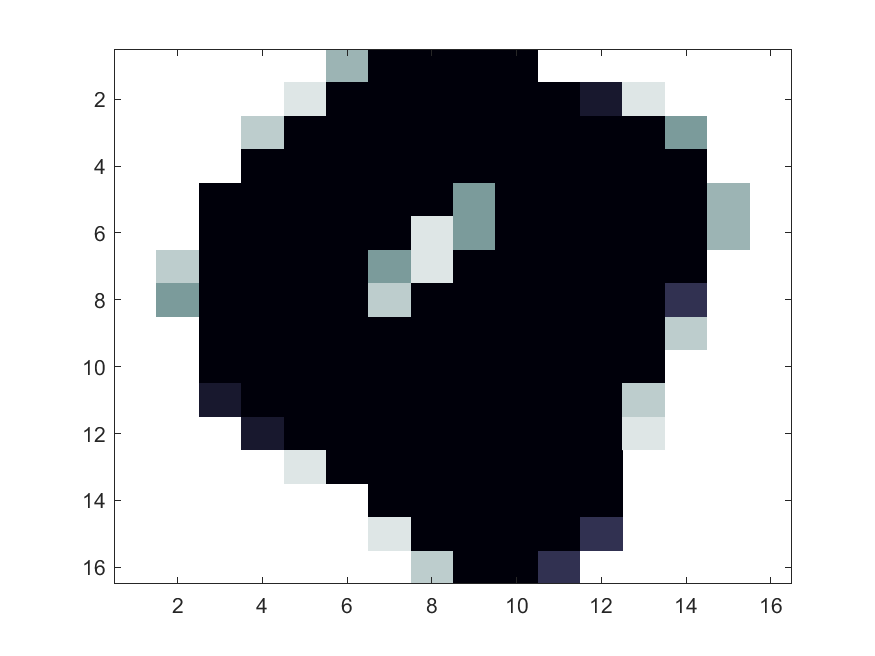
\includegraphics[width=0.25\textwidth]{fig/nine3_4.png}}
      
   \subfloat [pred=8]{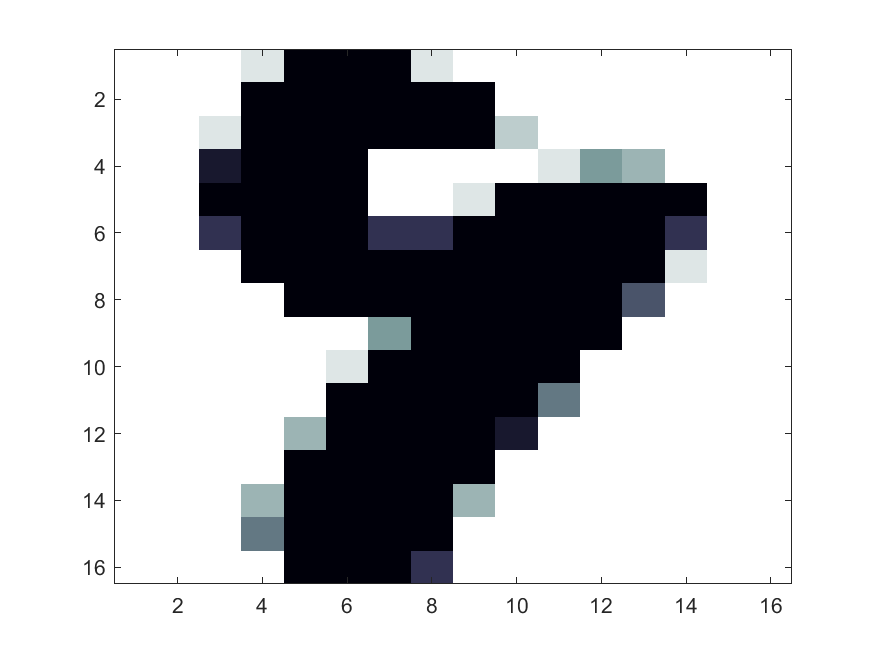
\includegraphics[width=0.25\textwidth]{fig/nine5_8.png}}
   \subfloat [pred=8]{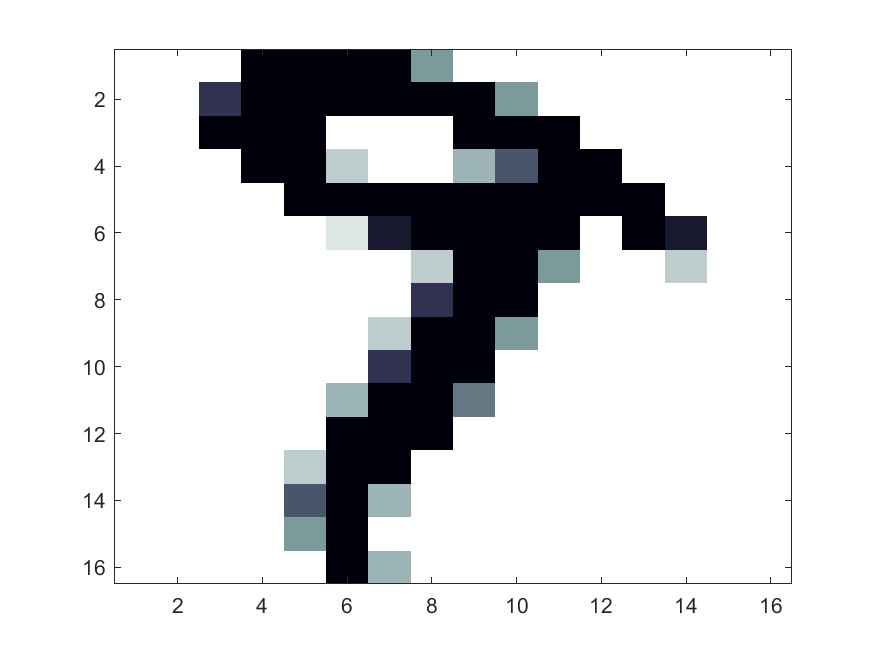
\includegraphics[width=0.25\textwidth]{fig/nine2_8.png}}
   \subfloat [pred=7]{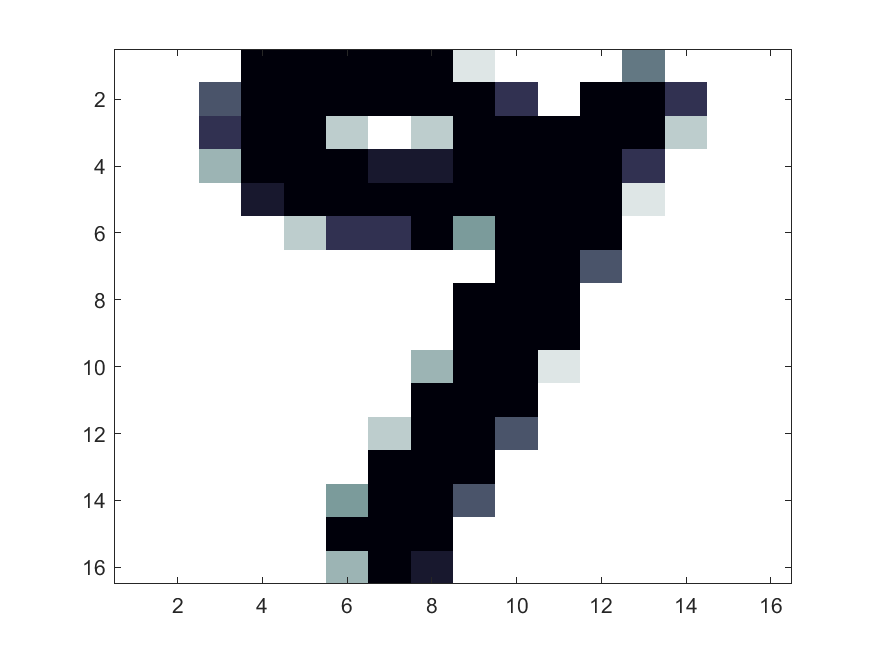
\includegraphics[width=0.25\textwidth]{fig/nine1_7.png}}
   \subfloat [pred=7]{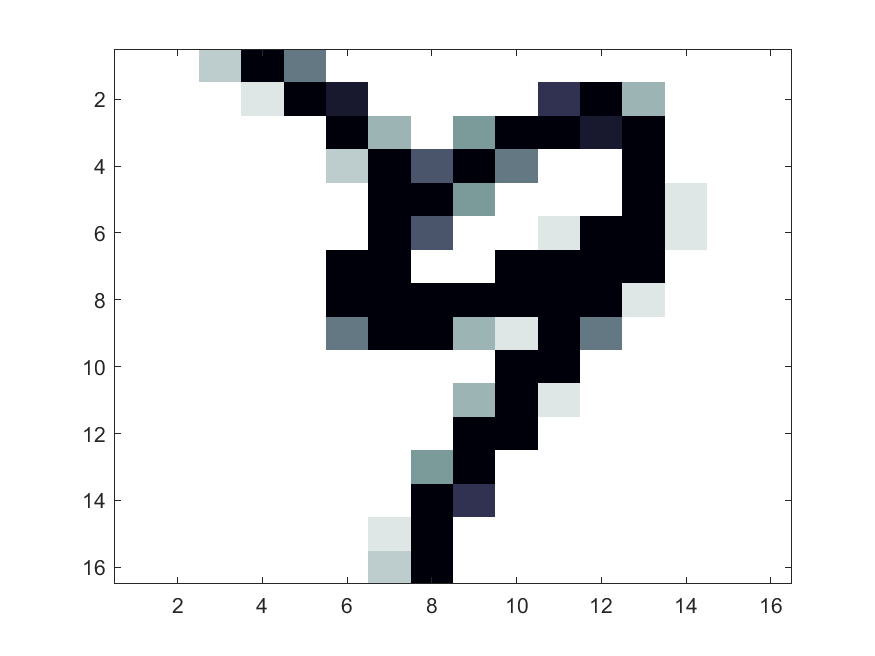
\includegraphics[width=0.25\textwidth]{fig/nine8_7.png}}
   \caption[]{Using 28 basis vector where the maximum accuracy is obtained for class of \textit{Number 9}, we draw the few instances where the images is classified incorrectly along with the wrong predication}
   \label{fig:nine}
\end{figure}






\newpage

\section*{Problem No.2} \label{sec:prob2}
\paragraph{Part A:}





\bibliography{../mybib}
\bibliographystyle{plain}
\end{document}